\chapter{New Algorithms for Social Recommendation}

After studying the results of the first trial, we made use of what we learned to design new algorithms to improve upon deficiencies of existing recommendation algorithms. Our goal in designing these algorithms was to address deficiencies in current SCF methods that was previously discussed at-length in Section~\ref{sec:objective}:

\begin{itemize}
\item {Non-feature-based user similarity}
% Note: potential for latent item information diffusion here
\item {Modeling direct user-user information diffusion}
\item {Restricted common interests}
\end{itemize}

We address these deficiencies by modifying the optimization objectives that were discussed in the previous chapter, creating new objective functions. We discuss these new objectives in the following sections.

\section{New Objective Components}
As in Chapter 4, we assume that the CF optimization objective decomposes into a sum of objective components as follows:

\begin{align}
\mathit{Obj} = \sum_i \lambda_i \mathit{Obj}_i
\end{align}

\subsection{Hybrid Objective ($\Obj_\phy$ )}

As specified in Chapter 1, one weakness of  MF methods is that they cannot model joint features over user and items, and hence the cannot model direct user-user information diffusion. Information diffusion models the unidirectional flow of links from one user to another (i.e., one user likes/shares what another user posts). We believe that this information will be useful for SCF, and is lacking in current SCF methods.

We fix this by introducing another objective component in addition to the standard MF objective, and this component serves as a simple linear regressor for such information diffusion observations. The resulting hybrid objective component becomes a combination of latent MF and linear regression objectives.

We make use of the $\f_{\x,\y}$ features detailed in Section~\ref{sec:dataset} to make the linear regressor. $\f_{\x,\y}$ models user-user information diffusion through the $F'_{\x,\y}$ indicator function of which of the user's friends have liked a particular link along with the user.

Using $\la \cdot,\cdot \ra$ to denote an inner product, we define a weight
vector $\w \in \R^F$ such that $\la \w, \f_{\x,\y} \ra = \w^T \f_{\x,\y}$ is the prediction of the system. The objective of the linear regression component is therefore

\begin{align*}
\sum_{(\x,\y) \in D} \frac{1}{2} (R_{\x,\y} - [\sigma] \w^T \f_{\x,\y})^2
\end{align*}

We combine the output of the linear regression objective with the Matchbox output $[\sigma] \x^T U^T V y$, to get a hybrid objective component. The full objective function for this hybrid model is

\begin{align}
\sum_{(\x,\y) \in D} \frac{1}{2} (R_{\x,\y} - [\sigma] \w^T \f_{\x,\y} - [\sigma] \x^T U^T V y)^2
\end{align}

\subsection{L2 $\w$ Regularization ($ \Obj_\rw$)}

In the same manner as $U$ and $V$, it is important to regularize the free parameter $\w$ to prevent overfitting in
the presence of sparse data. This can again be done with the
$L_2$ regularizer that models a prior of $0$ on the parameters. The objective component for the L2 regularizer for $\w$ is:

\begin{align}
\frac{1}{2} \| \w \|_2^2 = \frac{1}{2} \w^T \w
\end{align}

\subsection{Social Spectral Regularization ($\Obj_\rss$)}

As we did with the Social Regularization method in Section~\ref{sec:SocRec}, we build on ideas used in Matchbox~\cite{matchbox} to extend social spectral regularization~\cite{sr,rrmf} by incorporating user features into the objective. The objective function for our extension to social spectral regularization is:

\begin{align}
\sum_{\x} & \sum_{\z \in \mathit{friends}(\x)} \frac{1}{2} S^+_{\x,\z} \| U\x - U\z \|_2^2 \nonumber \\
& = \sum_{\x} \sum_{\z \in \mathit{friends}(\x)} \frac{1}{2} S^+_{\x,\z} \| U (\x - \z) \|_2^2 \nonumber \\
& = \sum_{\x} \sum_{\z \in \mathit{friends}(\x)} \frac{1}{2} S^+_{\x,\z} (\x - \z)^T U^T U (\x - \z)
\end{align}

\begin{comment}
\subfive Note: standard spectral regularization assumes $S^+_{\x,\z} \in [0,1]$;
however we may also want to try $S_{\x,\z}$ since a negative value actively
encourages the latent spaces to oppose each other, which may be desired.
\end{comment}

\subsection{Social Co-preference Regularization ($\Obj_\rsc$)}
\label{sec:rsc}

A crucial aspect missing from other SCF methods is that while two users may not be globally similar or opposite 
in their preferences, there may be sub-areas of their interests which can be correlated to each other.
For example, two friends may have similar interests concerning music, but 
different interests concerning politics.  The social co-preference regularizers
aim to learn such selective co-preferences. The motivation is to constrain users $\x$
and $\z$ who have similar or opposing
preferences to be similar or opposite in the same latent latent space
relevant to item $\y$.  

We use $\la \cdot, \cdot \ra_{\bullet}$ to denote a re-weighted inner product. The purpose of this inner product is to tailor the latent space similarities or dissimilarities between users to specific sets of items. This fixes the issue detailed in the previous paragraph by allowing users $\x$
and $\z$ to be similar or opposite in the same latent latent space
relevant only to item $\y$.  

The objective component for 
social co-preference regularization along with its expanded form is

\begin{align}
\sum_{(\x,\z,\y) \in C} & \frac{1}{2} (P_{\x,\z,\y} - \la U\x, U\z \ra_{V\y})^2 \nonumber \\
& = \sum_{(\x,\z,\y) \in C} \frac{1}{2} (P_{\x,\z,\y} - \x^T U^T \diag(V\y) U \z)^2
%= & \sum_{(\x,\z,\y) \in C}  \frac{1}{2} (P_{\x,\z,\y} - \sum_{k=1}^K (U\x)_k (U\z)_k (V\y)_k )^2 
\end{align}


\subsection{Social Co-preference Spectral Regularization ($\Obj_\rscs$)}
This is the same as the social co-preference regularization above, except that it uses the spectral regularizer format for 
learning the co-preferences.

 We use $\| \cdot \|_{2,\bullet}$ to denote a re-weighted $L_2$ norm. The reweighing of this norm servers the same purpose as the re-weighted inner product in Section~\ref{sec:rsc}, it tailors the similarities or dissimilarities between users to specific sets of items. This allows users $\x$
and $\z$ to be similar or opposite in the same latent latent space
relevant only to item $\y$.  
 
 The objective component for
 social co-preference spectral regularization along with its expanded form is
 
\begin{align}
\sum_{(\x,\z,\y) \in C} & \frac{1}{2} P_{\x,\z,\y} \| U\x - U\z \|_{2,V\y}^2 \nonumber \\
& = \sum_{(\x,\z,\y) \in C} \frac{1}{2} P_{\x,\z,\y} \| U (\x - \z) \|_{2,V\y}^2 \nonumber \\
& = \sum_{(\x,\z,\y) \in C} \frac{1}{2} P_{\x,\z,\y} (\x - \z)^T U^T \diag(V\y) U (\x - \z)
%= & \sum_{\x} \sum_{\z \neq \x} \sum_{\y} \frac{1}{2} P_{\x,\z,\y} \sum_{k=1}^K \big( \left[ (U\x)_k - (U\z)_k \right] (V\y)_k \big)^2
\end{align}

\subsection{Derivatives}
As before, we seek to optimize sums of the above objectives and will use
gradient descent for this purpose. Please see The Matrix Cookbook~\cite{matrix} for more details on the matrix derivative identities used in the following calculations.
We again use the following useful abbreviations:

\begin{align*}
\s & = U \x \qquad \s_{k} = (U \x)_{k}; \; k=1\ldots K\\
\t & = V \y \qquad \t_{k} = (V \y)_{k}; \; k=1\ldots K
\end{align*}

The derivatives for the hybrid objective functions as well as the new social regularizers are:

\begin{itemize}

\begin{comment}
\item {\bf Explicit Linear CBF}:
\begin{align*}
\frac{\partial}{\partial \w} \Obj_\pcbf & = \frac{\partial}{\partial \w} \sum_{(\x,\y) \in D} \frac{1}{2} \left( \underbrace{(R_{\x,\y} - [\sigma] \overbrace{\w^T \f_{\x,\y}}^{o_{\x,\y}})}_{\delta_{\x,\y}} \right)^2\\
& = \sum_{(\x,\y) \in D} \delta_{\x,\y} \frac{\partial}{\partial \w} - [\sigma] \w^T \f_{\x,\y}\\
& = - \sum_{(\x,\y) \in D} \delta_{\x,\y} [\sigma(o_{\x,\y}) (1 - \sigma(o_{\x,\y}))] \f_{\x,\y}
\end{align*}
\end{comment}

\item {\bf Hybrid}:
\begin{align*}
\frac{\partial}{\partial \w} \Obj_\phy & = \frac{\partial}{\partial \w} \sum_{(\x,\y) \in D} \frac{1}{2} \left( \underbrace{R_{\x,\y} - [\sigma] \overbrace{\w^T \f_{\x,\y}}^{o^1_{\x,\y}} - [\sigma] \x^T U^T V\y}_{\delta_{\x,\y}} \right)^2 \\
& = \sum_{(\x,\y) \in D} \delta_{\x,\y} \frac{\partial}{\partial \w} - [\sigma] \w^T \f_{\x,\y} \\
& = - \sum_{(\x,\y) \in D} \delta_{\x,\y} [\sigma(o^1_{\x,\y}) (1 - \sigma(o^1_{\x,\y}))] \f_{\x,\y} 
\end{align*}
\begin{align*}
\frac{\partial}{\partial U} \Obj_\phy & = \frac{\partial}{\partial U} \sum_{(\x,\y) \in D} \frac{1}{2} \left( \underbrace{R_{\x,\y} - [\sigma] \w^T \f_{\x,\y} - [\sigma] \overbrace{\x^T U^T V\y}^{o^2_{\x,\y}}}_{\delta_{\x,\y}}\right)^2 \\
& = \sum_{(\x,\y) \in D} \delta_{\x,\y} \frac{\partial}{\partial U} - [\sigma] \x^T U^T V\y \\
& = - \sum_{(\x,\y) \in D} \delta_{\x,\y} [\sigma(o^2_{\x,\y}) (1 - \sigma(o^2_{\x,\y}))] \t \x^T\\
%\end{align*}
%\begin{align*}
\frac{\partial}{\partial V} \Obj_\phy & = \frac{\partial}{\partial V} \sum_{(\x,\y) \in D} \frac{1}{2} \left( \underbrace{R_{\x,\y} - [\sigma] \w^T \f_{\x,\y} - [\sigma] \overbrace{\x^T U^T V\y}^{o^2_{\x,\y}}}_{\delta_{\x,\y}}\right)^2 \\
& = \sum_{(\x,\y) \in D}  \delta_{\x,\y} \frac{\partial}{\partial V} - [\sigma] \x^T U^T V\y \\
& = - \sum_{(\x,\y) \in D}  \delta_{\x,\y} [\sigma(o^2_{\x,\y}) (1 - \sigma(o^2_{\x,\y}))] \s \y^T \\
\end{align*}

\item {\bf $L_2$ $\w$ regularization}:
\begin{align*}
\frac{\partial}{\partial \w} \Obj_\rw & = \frac{\partial}{\partial \w} \frac{1}{2} \w^T \w\\
& = \w
\end{align*}

\item {\bf Social spectral regularization}:
\begin{align*}
\frac{\partial}{\partial U} \Obj_\rss & = \frac{\partial}{\partial U} \sum_{\x} \sum_{\z \in \mathit{friends}(\x)} \frac{1}{2} S^+_{\x,\z} (\x - \z)^T U^T U (\x - \z) \\
& = \sum_{\x} \sum_{\z \in \mathit{friends}(\x)} \frac{1}{2} S^+_{\x,\z} U ((\x - \z)(\x - \z)^T + (\x - \z)(\x - \z)^T)\\
& = \sum_{\x} \sum_{\z \in \mathit{friends}(\x)} S^+_{\x,\z} U (\x - \z)(\x - \z)^T
\end{align*}
\end{itemize}
Before we proceed to the final derivatives, we define one additional
vector abbreviation: 
\begin{align*}
\r & = U \z \qquad \r_{k} = (U \z)_{k}; \; k=1\ldots K .
\end{align*}
\begin{itemize}
\item {\bf Social co-preference regularization}:
\begin{align*}
\frac{\partial}{\partial U} \Obj_\rsc & = \frac{\partial}{\partial U} \sum_{(\x,\z,\y) \in C} \frac{1}{2} \left( \underbrace{P_{\x,\z,\y} - \x^T U^T \diag(V\y) U \z}_{\delta_{\x,\z,\y}} \right)^2\\
& = \sum_{(\x,\z,\y) \in C} \delta_{\x,\z,\y} \frac{\partial}{\partial U} - \x^T U^T \diag(V\y) U \z \\
%%%%%%%%%%%%%%%%%%%%%%%%%%%%%%%%%%%%%%%%%%%%%%%%%%%%%%%%%%%%%%%%%%%%%%%%
%& = \delta \frac{\partial}{\partial U} - \tr(\diag(\x) U^T \diag(V\y) U \diag(\z)) \\
%& = - \delta \diag(\z) \diag(\x) U^T \diag(V\y) + \diag(\x)^T \diag(\z)^T U^T \diag(V\y)^T\\
%& = - \delta \diag(V\y)^T U \diag(\x)^T \diag(\z)^T + \diag(V\y)^T U \diag(\z)^T \diag(\x)^T\\
%& = - \delta \diag(V\y)^T U (\diag(\x) \diag(\z) + \diag(\z) \diag(\x)) \\
%& = - \delta \diag(V\y)^T U (\z \x^T + \x \z^T) \\
%%%%%%%%%%%%%%%%%%%%%%%%%%%%%%%%%%%%%%%%%%%%%%%%%%%%%%%%%%%%%%%%%%%%%%%%
% Found it, see here for direct derivative: http://www.ee.ic.ac.uk/hp/staff/dmb/matrix/calculus.html
& = - \sum_{(\x,\z,\y) \in C} \delta_{\x,\z,\y} (\diag(V\y)^T U \x \z^T + \diag(V\y) U \z \x^T)\\ % \diag(V\y)^T = \diag(V\y)
& = - \sum_{(\x,\z,\y) \in C} \delta_{\x,\z,\y} \diag(V\y) U (\x \z^T + \z \x^T)\\
\end{align*}
In the following, $\circ$ is the Hadamard elementwise product:
\begin{align*}
\frac{\partial}{\partial V} \Obj_\rsc & = \frac{\partial}{\partial V} \sum_{(\x,\z,\y) \in C} \frac{1}{2} (P_{\x,\z,\y} - \x^T U^T \diag(V\y) U \z)^2\\
 & = \frac{\partial}{\partial V} \sum_{(\x,\z,\y) \in C} \frac{1}{2} \left( \underbrace{P_{\x,\z,\y} -  (\overbrace{U\x}^\s \circ \overbrace{U\z}^\r)^T V\y}_{\delta_{\x,\z,\y}} \right)^2\\
 & = \sum_{(\x,\z,\y) \in C} \delta_{\x,\z,\y} \frac{\partial}{\partial V} - (\s \circ \r)^T V\y\\
 & = - \sum_{(\x,\z,\y) \in C} \delta_{\x,\z,\y} (\s \circ \r) \y^T
\end{align*}
\item {\bf Social co-preference spectral regularization}:
\begin{align*}
\frac{\partial}{\partial U} \Obj_\rscs & = \frac{\partial}{\partial U} \sum_{(\x,\z,\y) \in C} \frac{1}{2} P_{\x,\z,\y} (\x - \z)^T U^T \diag(V\y) U (\x - \z)\\
& = \sum_{(\x,\z,\y) \in C} \frac{1}{2} P_{\x,\z,\y} \left( \diag(V\y)^T U (\x - \z) (\x - \z)^T \right.\\
& \left. \qquad \qquad \qquad \qquad + \diag(V\y) U (\x - \z) (\x - \z)^T \right)\\
& = \sum_{(\x,\z,\y) \in C} P_{\x,\z,\y} \diag(V\y) U (\x - \z) (\x - \z)^T\\
\frac{\partial}{\partial V} \Obj_\rscs & = \frac{\partial}{\partial V} \sum_{(\x,\z,\y) \in C} \frac{1}{2} P_{\x,\z,\y} (\x - \z)^T U^T \diag(V\y) U (\x - \z)\\
& = \frac{\partial}{\partial V} \sum_{(\x,\z,\y) \in C} \frac{1}{2} P_{\x,\z,\y} (U(\x-\z) \circ U(\x-\z))^T V\y\\
& = \frac{1}{2} \sum_{(\x,\z,\y) \in C} P_{\x,\z,\y} (U(\x-\z) \circ U(\x-\z)) \y^T
\end{align*}
\end{itemize}

Hence, for any choice of primary objective and one or more regularizers,
we simply add the derivatives for each of $\w$, $U$, and $V$
according to~\eqref{eq:sum_der}.

\section{Second Trial}

For the second online trial, we chose four algorithms again to randomly split between the LinkR application users. Social Matchbox was included again as a baseline since it was the best performing algorithm in the first trial. The distribution count of the algorithms to the users is shown in Table~\ref{tab:assigned2}

The four SCF algorithms are:

\begin{itemize}
\item{{\bf Social Matchbox (Soc. Mbox)} : Matchbox MF + Social Regularization +  L2 $U$ Regularization + L2 $V$ Regularization}
\item{{\bf Spectral Matchbox (Spec. Mbox)}: Matchbox MF + Social Spectral Regularization + L2 $U$ Regularization + L2 $V$ Regularization}
\item{{\bf Social Hybrid (Soc. Hybrid)}: Hybrid + Social Regularization + L2 $U$ Regularization + L2 $V$ Regularization + L2 $\w$ Regularization}
\item{{\bf Spectral Co-preference (Spec. CP)}: Matchbox MF + Social Co-preference Spectral Regularization + L2 $U$ Regularization + L2 $V$ Regularization}
\end{itemize}

\subsection{Online Results}
\label{sec:online2}

The online experiments were switched to the new algorithms on October 13, 2011. For the online results reported here, since the second live trial is still currently ongoing, we took a snapshot of the data as it was on October 22, 2011. The algorithms were randomly distributed among the 103 users who still had the LinkR application installed. The distribution of the algorithms to the users are show in Table~\ref{tab:assigned2}


\begin{table}[t!]
\centering
\begin{tabular}{| l | c |}
\hline
{\bf Algorithm} & {\bf Users} \\
\hline
Social Matchbox & 26\\
Spectral Matchbox  & 25 \\
Spectral Co-preference & 27 \\
Social Hybrid & 25 \\
\hline
\end{tabular}
\caption{Number of Users Assigned per Algorithm.}
\label{tab:assigned2}
\end{table}

Results shown in Figure~\ref{fig:online2} are the percentage of Like ratings and the percentage of Dislike ratings per algorithm stacked on top of each other with the Like ratings on top. 

First thing we note in Figure~\ref{fig:online2} is the decrease in performance for Social Matchbox, and in fact for all SCF algorithms in general. Except for Spectral Matchbox, they all received more Dislike ratings than Like ratings. What we noticed is that  of the recommendations being made in the week that we switched over to the new algorithms, the majority of the links were about Steve Jobs, who had died the week previously. We believe that the redundancy and lack of variety of the links being recommended caused an increase in the Dislike ratings being given by users on the recommended links. Taking out the skewed results that follows an unusual event such as this, the relative algorithm performance was better. 

\begin{figure}[t!]
\centering
\subfigure{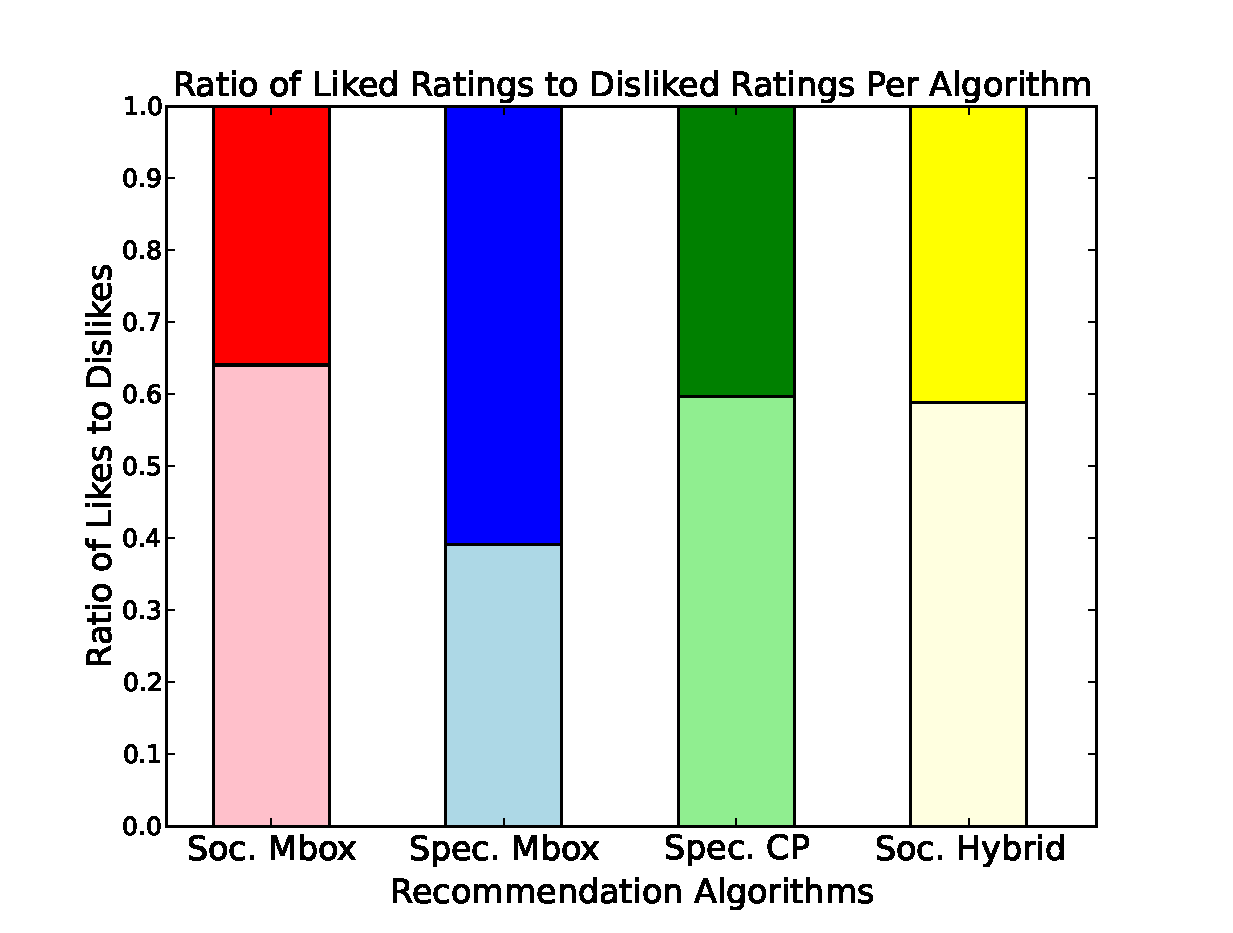
\includegraphics[scale=0.5]{img/live-likes2.eps}}
%\subfigure{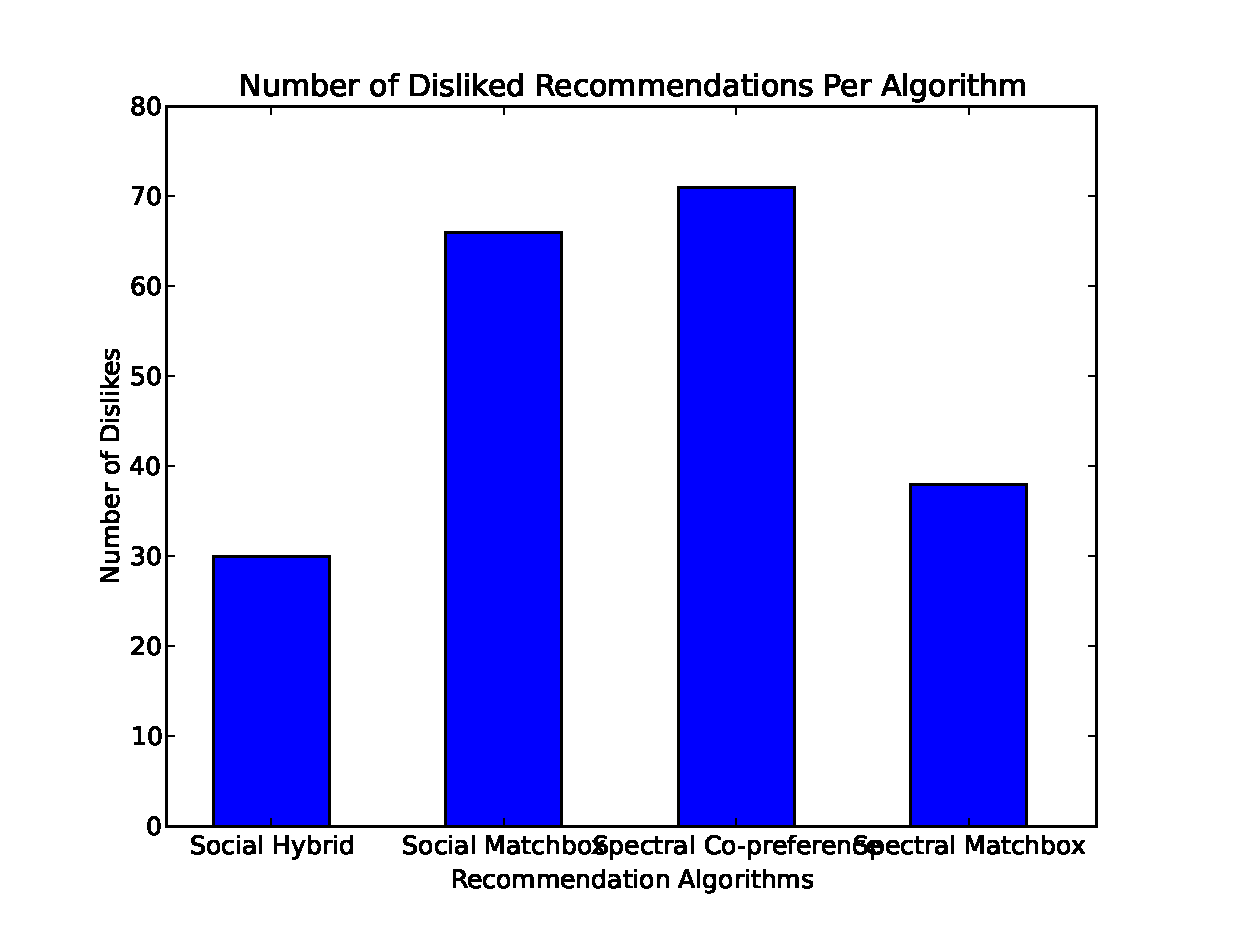
\includegraphics[scale=0.35]{img/live-dislikes2.eps}}
\caption{Results of online live trials. The percentage of Liked ratings are stacked on top of the percentage of Disliked ratings per algorithm. Spectral Matchbox achieved the highest ratio of likes to dislikes among the four algorithms. Spectral social regularization in general appears to be a better way to socially regularize compared to social regularization.}
\label{fig:online2}
\end{figure}

We again split the results again between friend link recommendations and non-friend link recommendations, with the results shown in Figure~\ref{fig:OnlineFriend2} being the percentage of Like ratings and the percentage of Dislike ratings per algorithm stacked on top of each other with the Like ratings on top.
 As shown Figure~\ref{fig:OnlineFriend2}, all four algorithms experienced significant performance drop in the number of likes when it came to recommending non-friend links. This reflects the results of the first trial. 
 
 \begin{comment}
 Additionally, the differences were more drastic with the two algorithms that uses the social regularization method: Social Matchbox and Social Hybrid. This, together with results of the first user trial, seems to confirm our earlier analysis that aside from Liking or Disliking a link just from the quality of the links being recommended, users are also more likely to like a link because a friend had posted it and more likely to dislike it because it came from a stranger.
\end{comment}

\begin{figure}[t!]
\centering
\subfigure{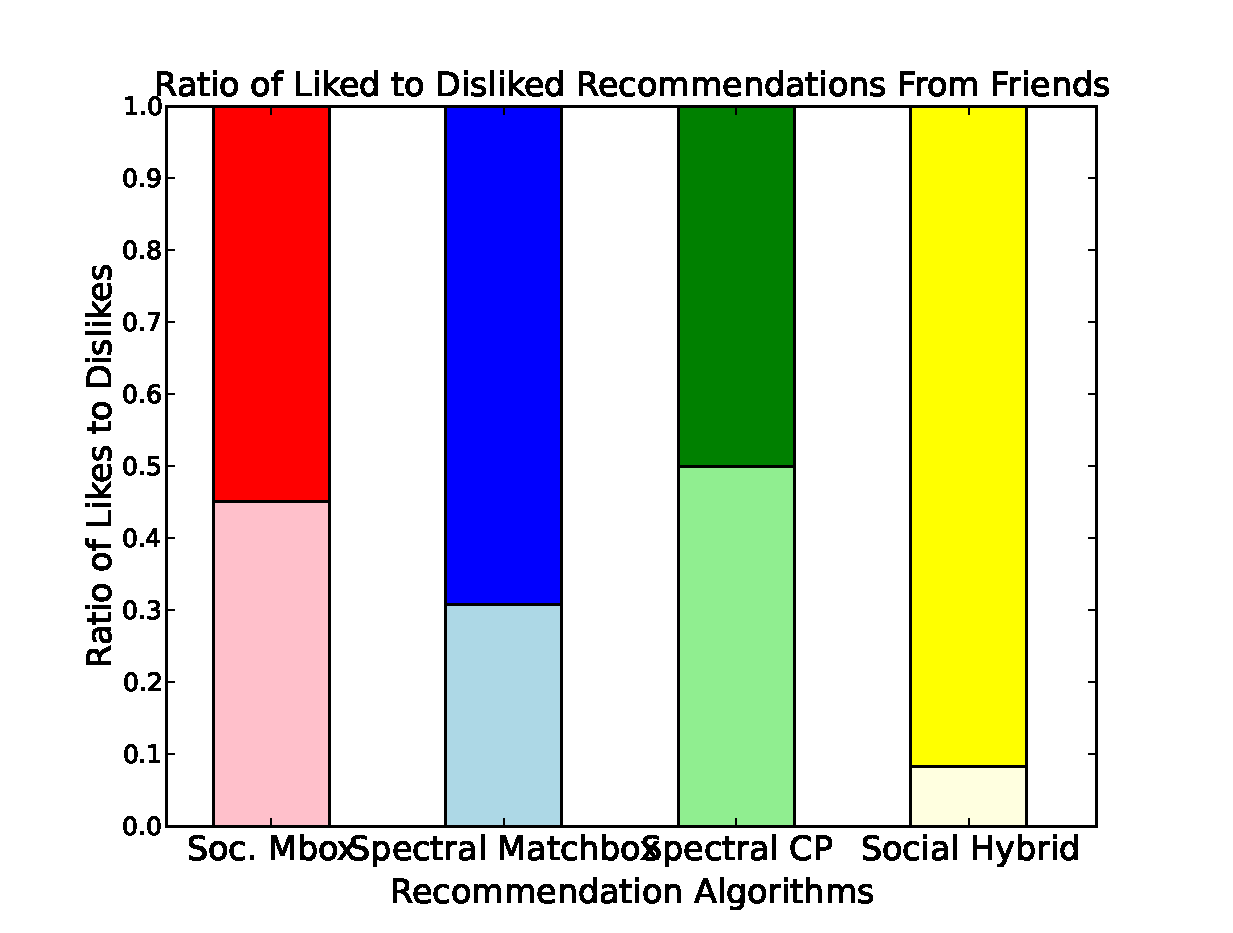
\includegraphics[scale=0.5]{img/live-friend-likes2.eps}}
\subfigure{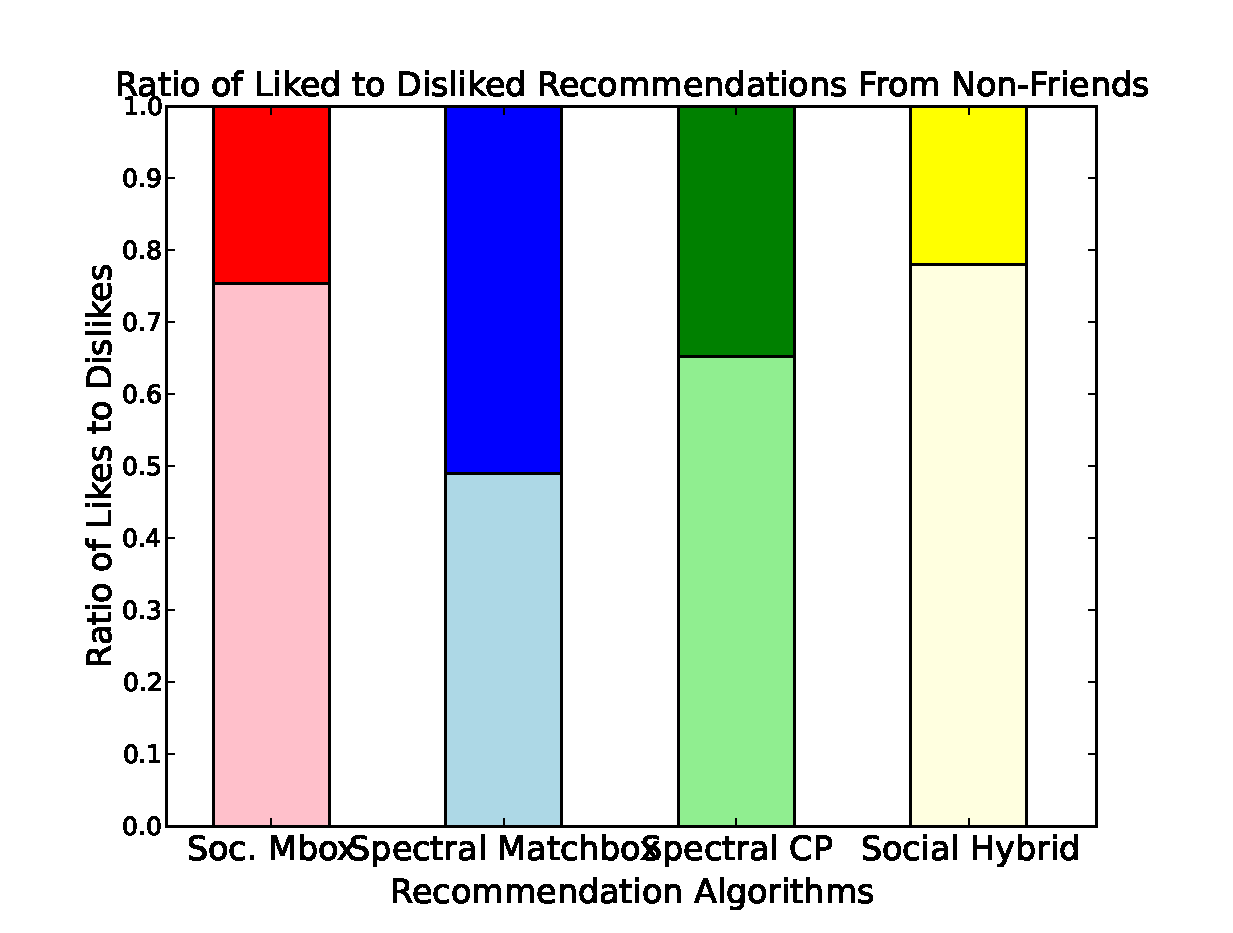
\includegraphics[scale=0.5]{img/live-nonfriend-likes2.eps}}
%\subfigure{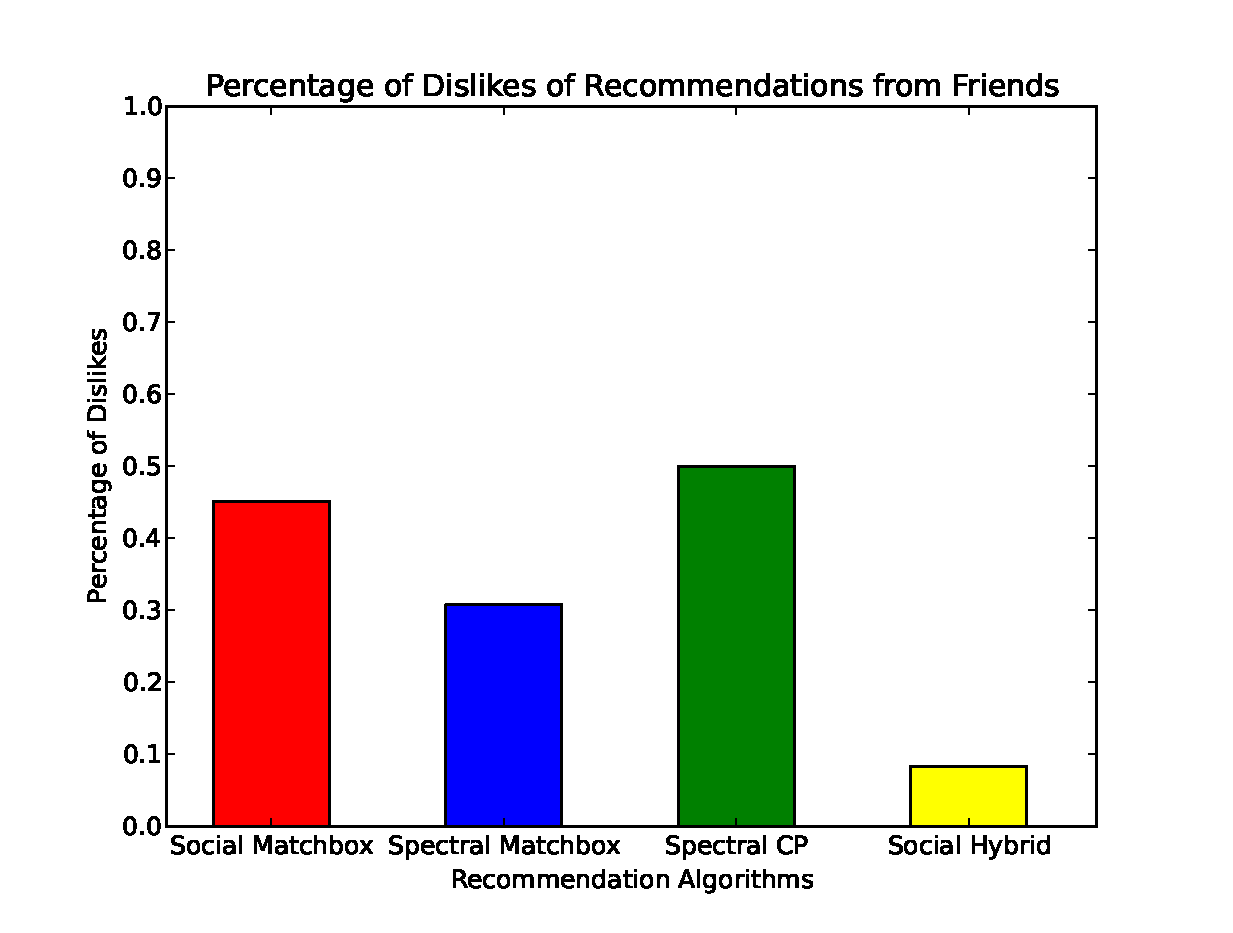
\includegraphics[scale=0.35]{img/live-friend-dislikes2.eps}}
%\subfigure{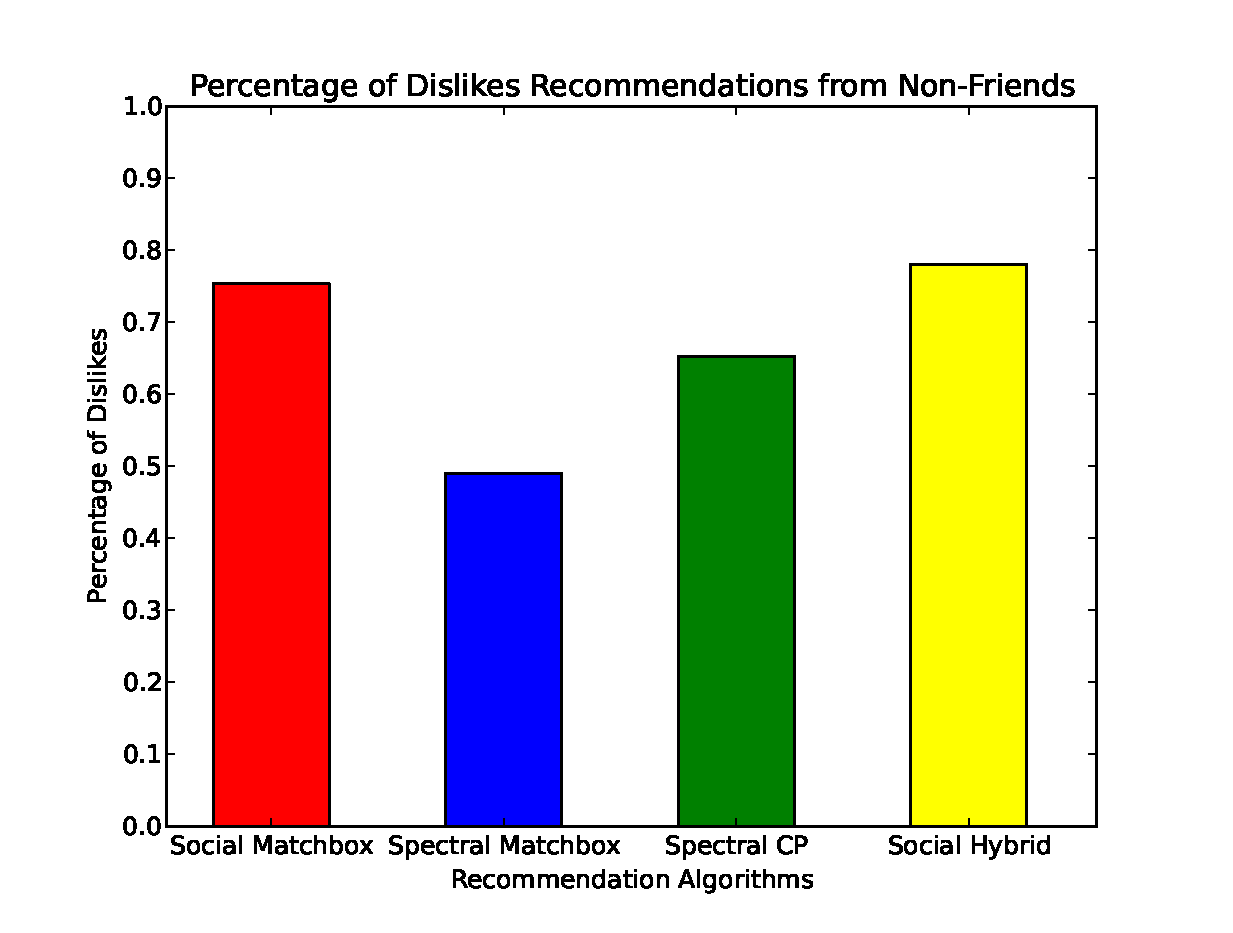
\includegraphics[scale=0.35]{img/live-nonfriend-dislikes2.eps}}
\caption{Results of the online live trials, split between friends and non-friends. As in the first trial, there is a significant drop in performance between recommending friend links and recommending non-friend links.}
\label{fig:OnlineFriend2}
\end{figure}

We note the following observations from the results shown in Figures \ref{fig:online2} and \ref{fig:OnlineFriend2}:

\begin{itemize}
\item{Compared to the other algorithms, Spectral Matchbox achieved the best ratio of likes to dislikes as seen, as seen in Figure~\ref{fig:online2}. Combined with the results for Spectral Co-preference, Spectral social regularization in general appears to be a better way to socially regularize compared to social regularization. This comparison holds even when the results are split between friend links recommendations and non-friend links recommendations, as seen in Figure~\ref{fig:OnlineFriend2}.}

\item{When looking at just the friend link recommendations in Figure~\ref{fig:OnlineFriend2}, Social Hybrid was the best performing algorithm. This result comes from the user-user information diffusion among its friends that Social Hybrid learns, which could not be learned by the other SCF algorithms. Learning information diffusion thus helps when it comes to building better SCF algorithms.}

\item{Spectral Co-preference didn't do well on friend link recommendations, however it did better on the non-friend link recommendations. When it comes to recommending friend links, friend interaction information coming through social regularizer seems more important than implicit co-likes information provided by the co-preference regularizer. When there is no social interaction information such as with non-friend links, co-preference methods with its implicit co-likes information appear much better than just vanilla collaborative filtering at projecting users into subspaces of common interest.}
\end{itemize}

\section{Offline Results}

Aside from the online user trial, we also evaluate the algorithms using the mean average precision metric discussed in Section 3.3. We note the following observations from the results shown in Figures \ref{fig:passive2}, \ref{fig:active2}, and \ref{fig:union2}:

\begin{itemize}
\item{Most results are not statistically significant.}

\item{In Figure~\ref{fig:union2}, when training UNION and testing on APP-USER-ACTIVE-FRIEND, Social Hybrid gets the score on the MAP metric. This reflects the results of the live user trial in Section~\ref{sec:online2}.}

\item{ In Figure~\ref{fig:active2}, when training on ACTIVE and testing on APP-USER-ACTIVE-NON-FRIEND, Spectral Co-preference shows slightly better (though not statistically significant) performance than when testing on APP-USER-ACTIVE-FRIEND. This also reflects the results of the live user trial in Section~\ref{sec:online2}. The explicit dislikes of the Active data allow the co-preference regularizer to learn the Dislike data better.}

\item{The better performance of the social spectral regularization methods in the live user trials do not show in the offline experiments. This may be caused by the difference in the dataset size between the live user trials and the offline experiments, which affected optimal parameter settings for the offline experiments. Further tuning of the parameters may cause the social spectral regularization methods to perform better}

\item{Another reason may be that perhaps the MAP metric isn't the best metric that correlates with human performance evaluation, and some other metric that we could have used instead may better reflect the results of live user trials.}
\end{itemize}

%When training on the UNION dataset, we can see the same general worsening of performance between the results of testing on APP-USER-ACTIVE-FRIENDS and APP-USER-ACTIVE-NON-FRIENDS. 

\begin{figure}[t!]
\centering
\subfigure{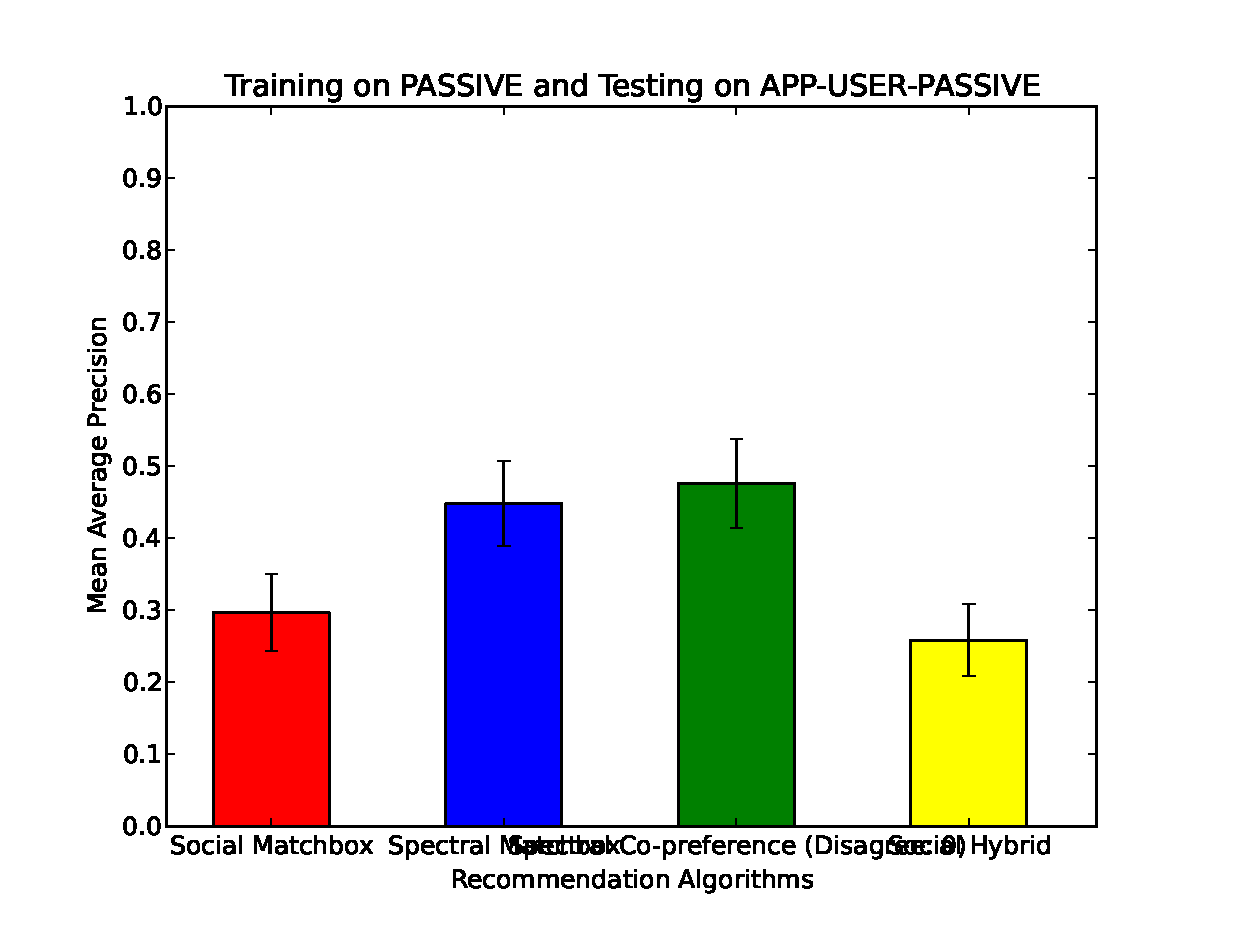
\includegraphics[scale=0.35]{img/Passive_App-User-Passive2.eps}}
\subfigure{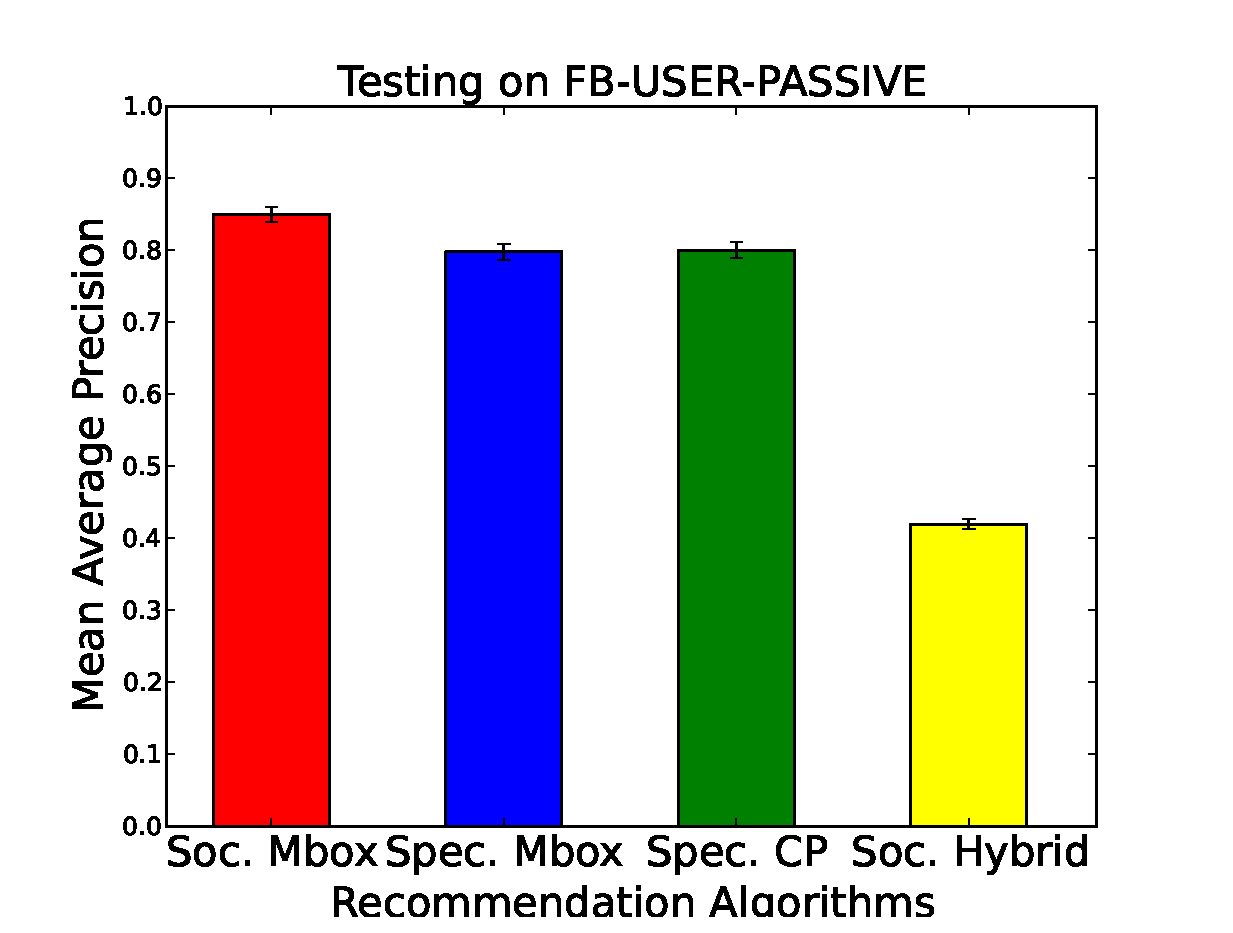
\includegraphics[scale=0.35]{img/Passive_FB-User-Passive2.eps}}
\subfigure{\includegraphics[scale=0.35]{img/Passive_App-User-active-all2.eps}}
\subfigure{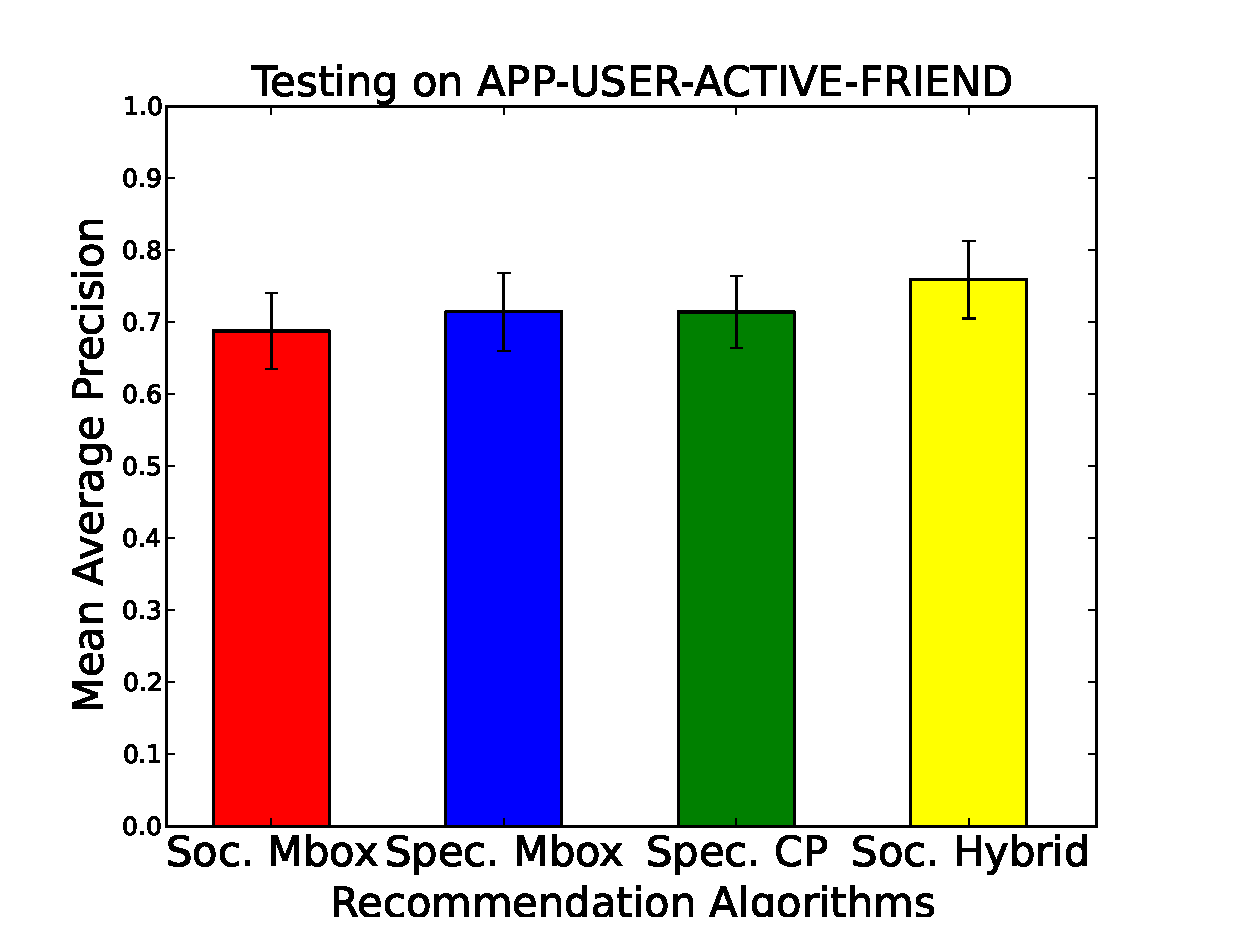
\includegraphics[scale=0.35]{img/Passive_App-User-Active-Friends2.eps}}
\subfigure{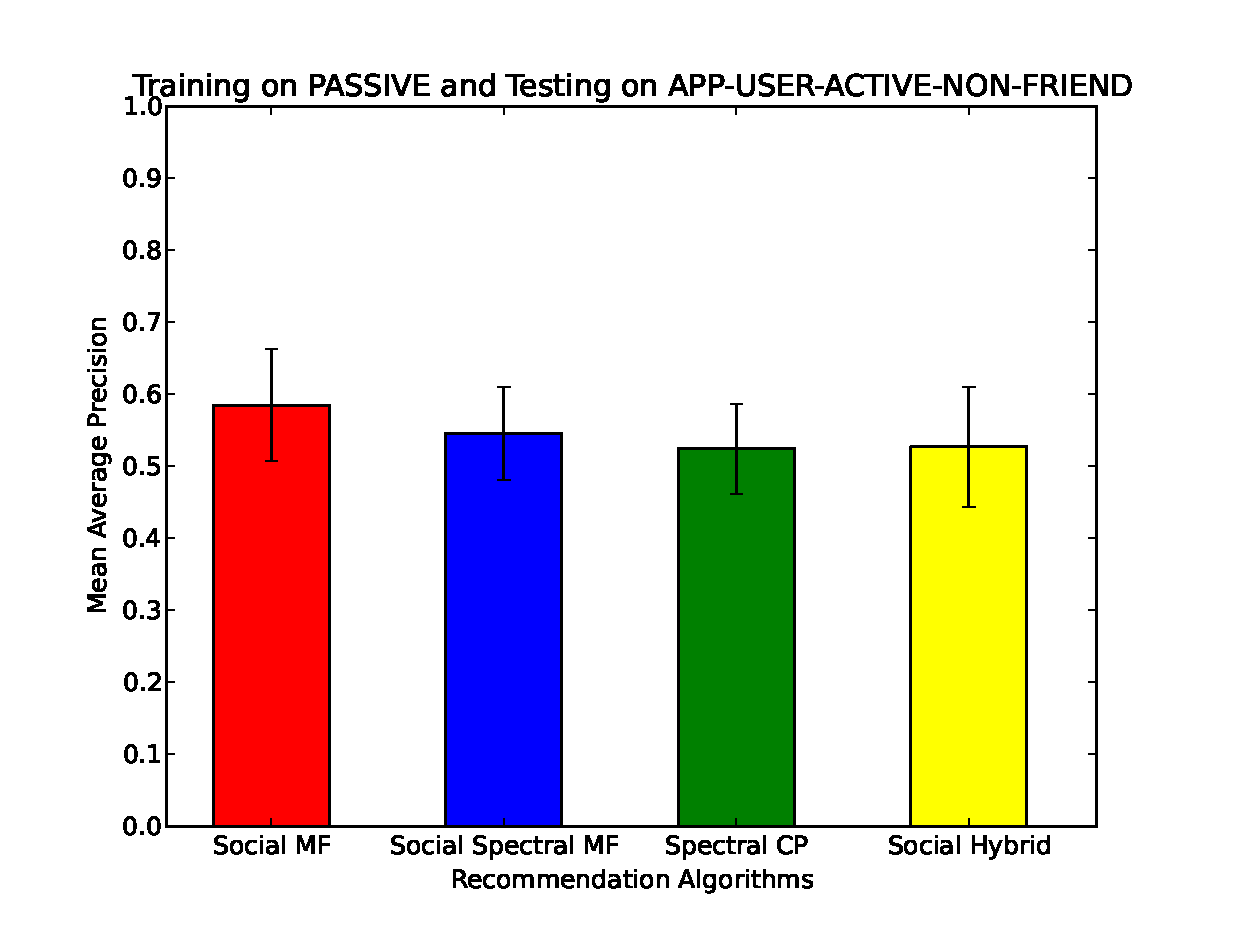
\includegraphics[scale=0.35]{img/Passive_App-User-Active-NonFriends2.eps}}
\caption{Results of training on Passive data}
\label{fig:passive2}
\end{figure}

\begin{figure}[t!]
\centering
\subfigure{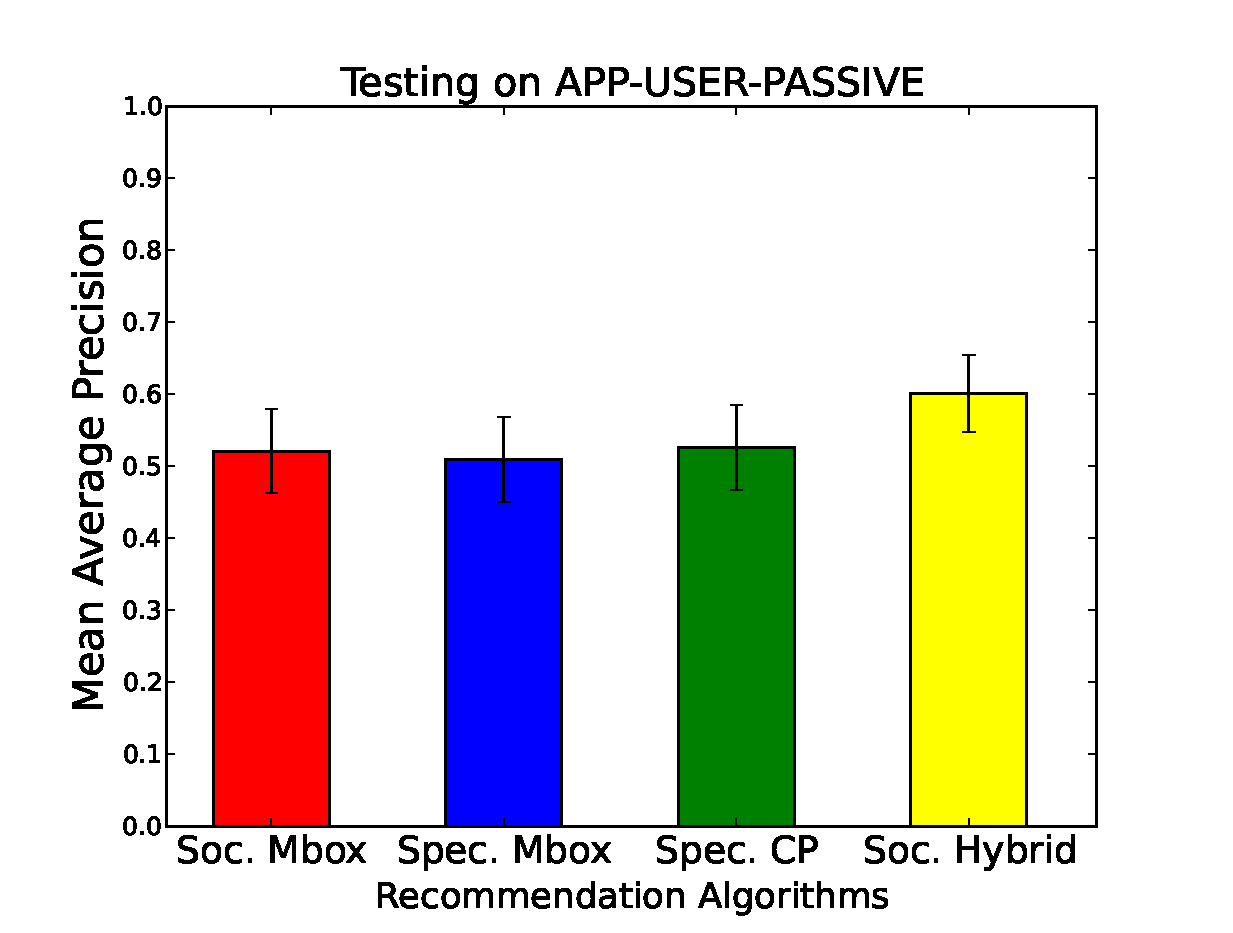
\includegraphics[scale=0.35]{img/Active_App-User-Passive2.eps}}
\subfigure{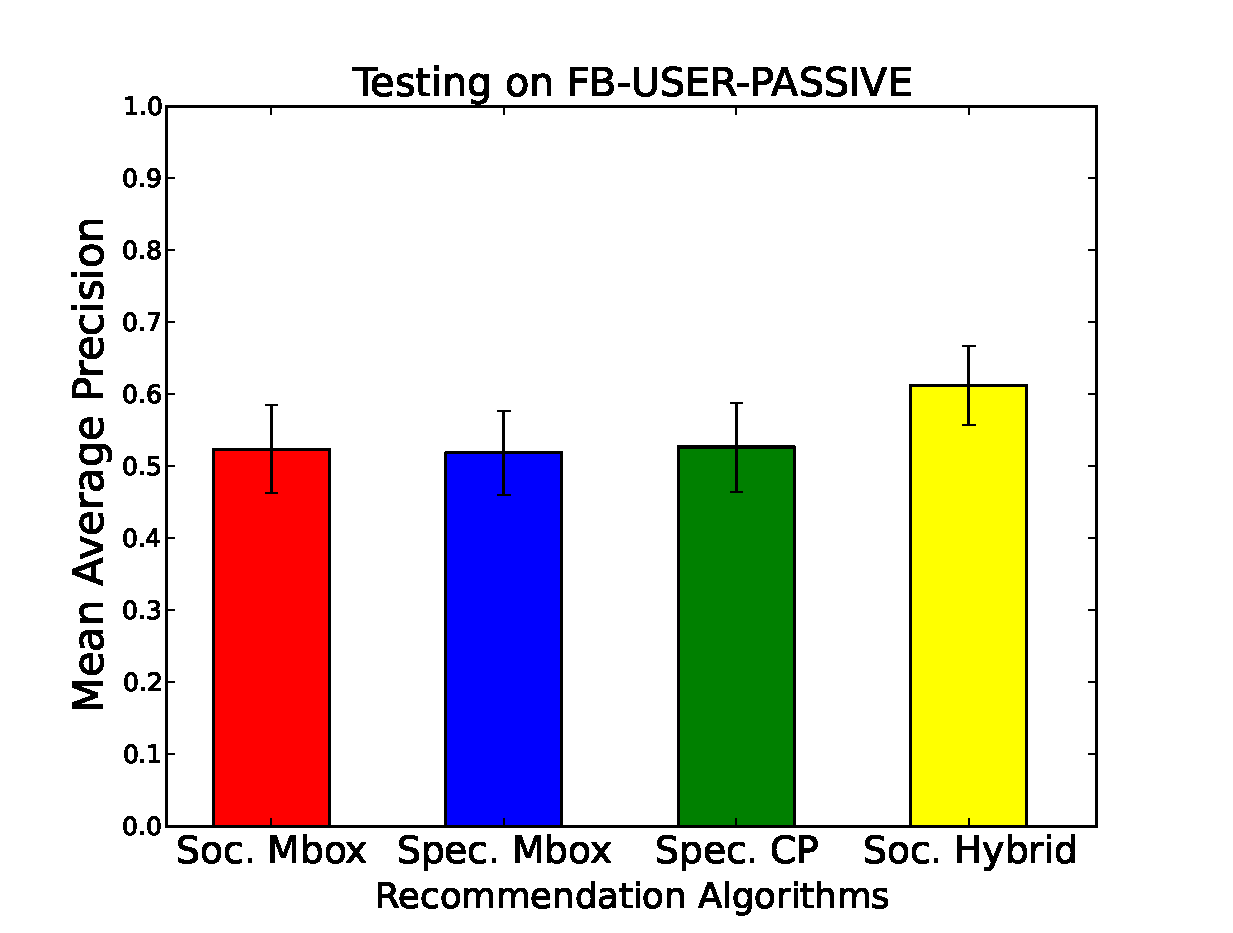
\includegraphics[scale=0.35]{img/Active_FB-User-Passive2.eps}}
\subfigure{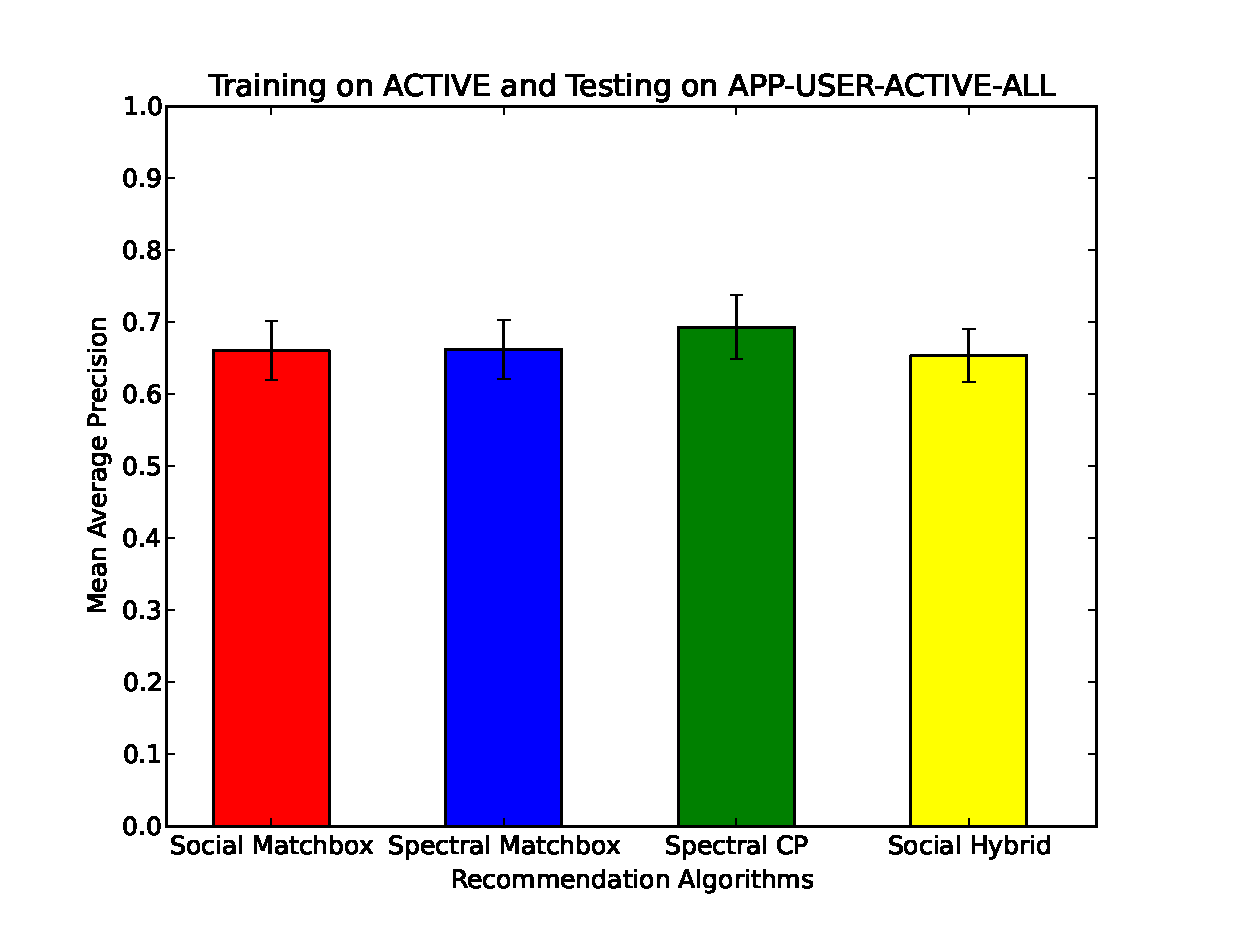
\includegraphics[scale=0.35]{img/Active_App-User-Active-All2.eps}}
\subfigure{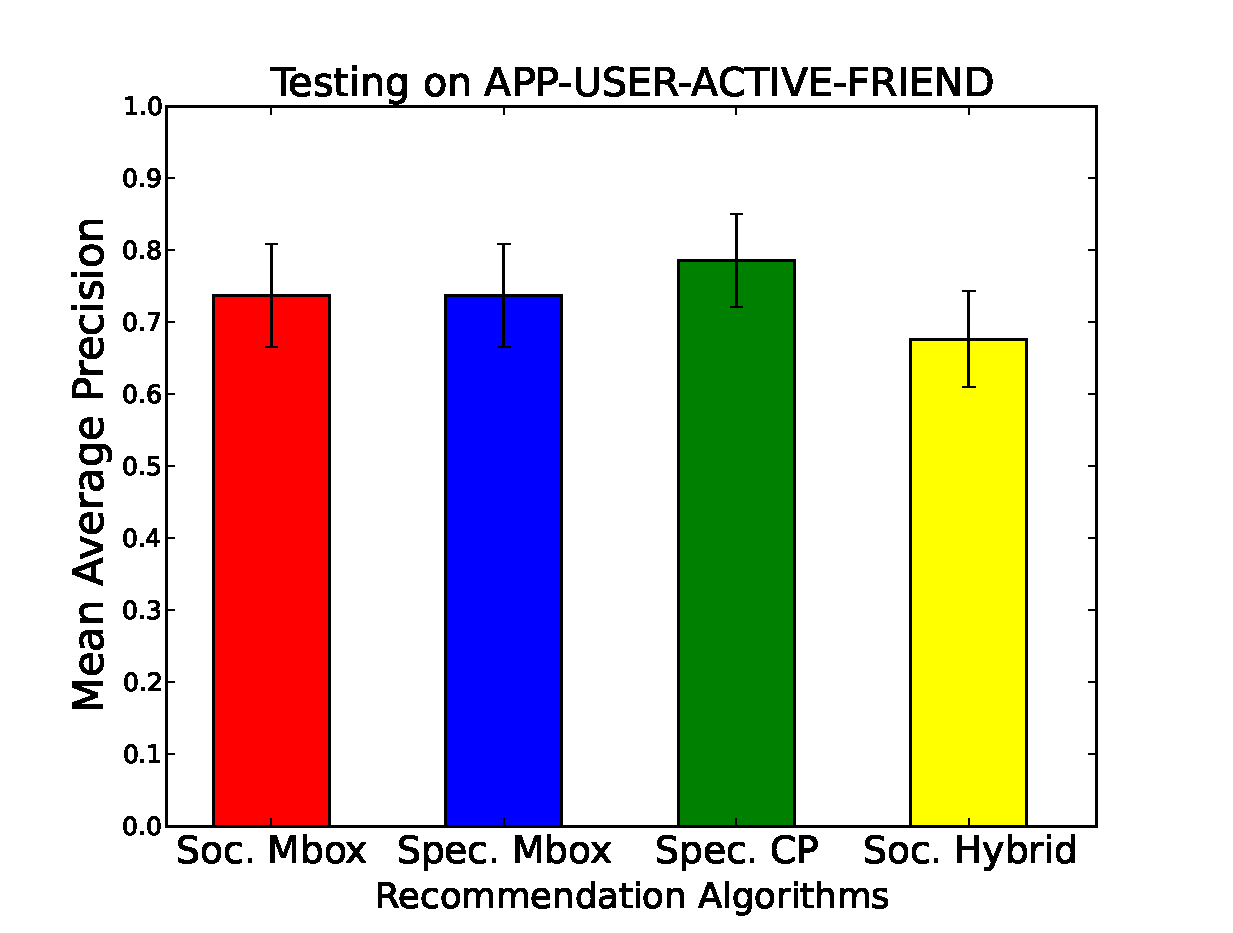
\includegraphics[scale=0.35]{img/Active_App-User-Active-Friends2.eps}}
\subfigure{\includegraphics[scale=0.35]{img/Active_App-User-Active-Nonfriends2.eps}}
\caption{Results of training on Active data}
\label{fig:active2}
\end{figure}

\begin{figure}[t!]
\centering
\subfigure{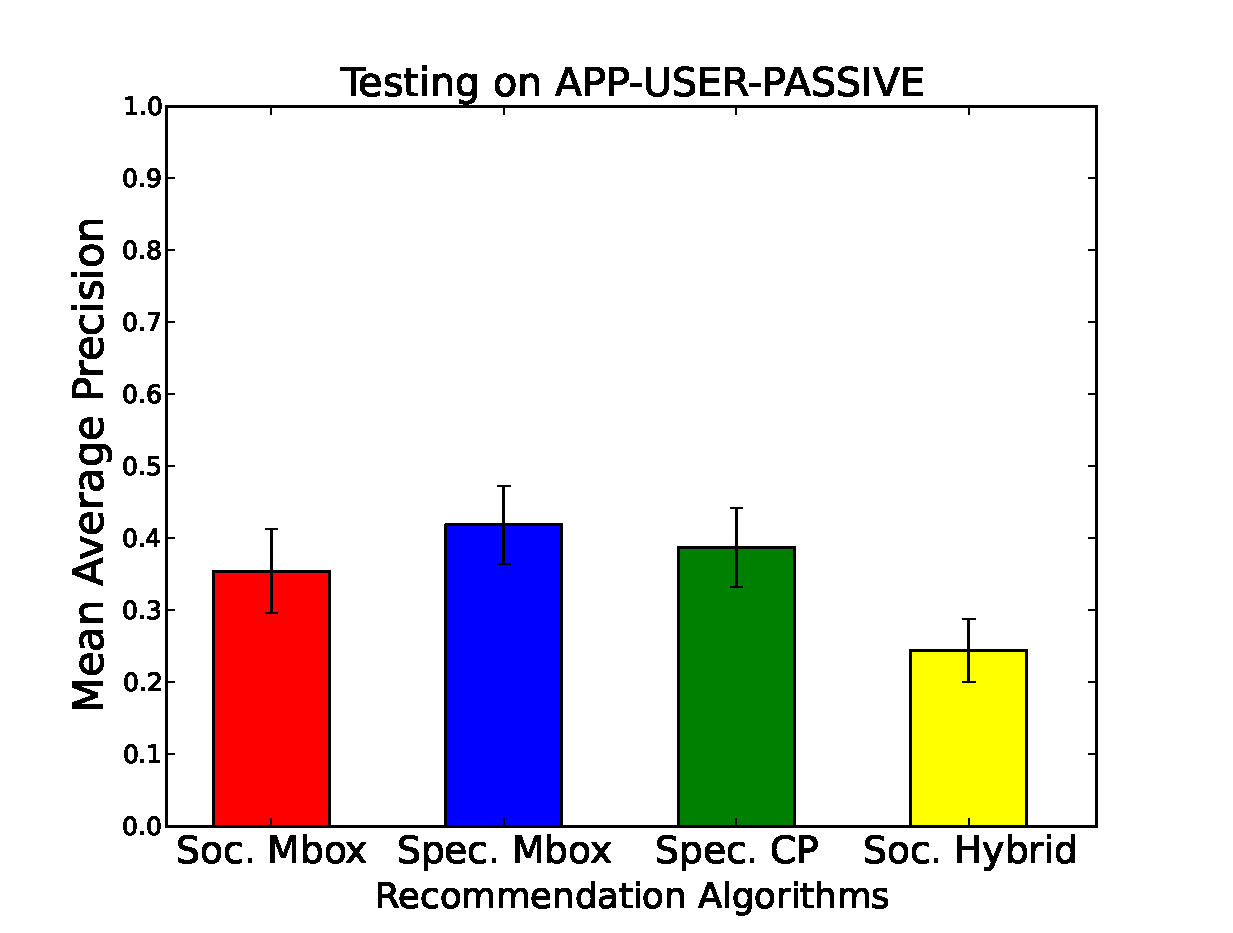
\includegraphics[scale=0.35]{img/Union_App-User-Passive2.eps}}
\subfigure{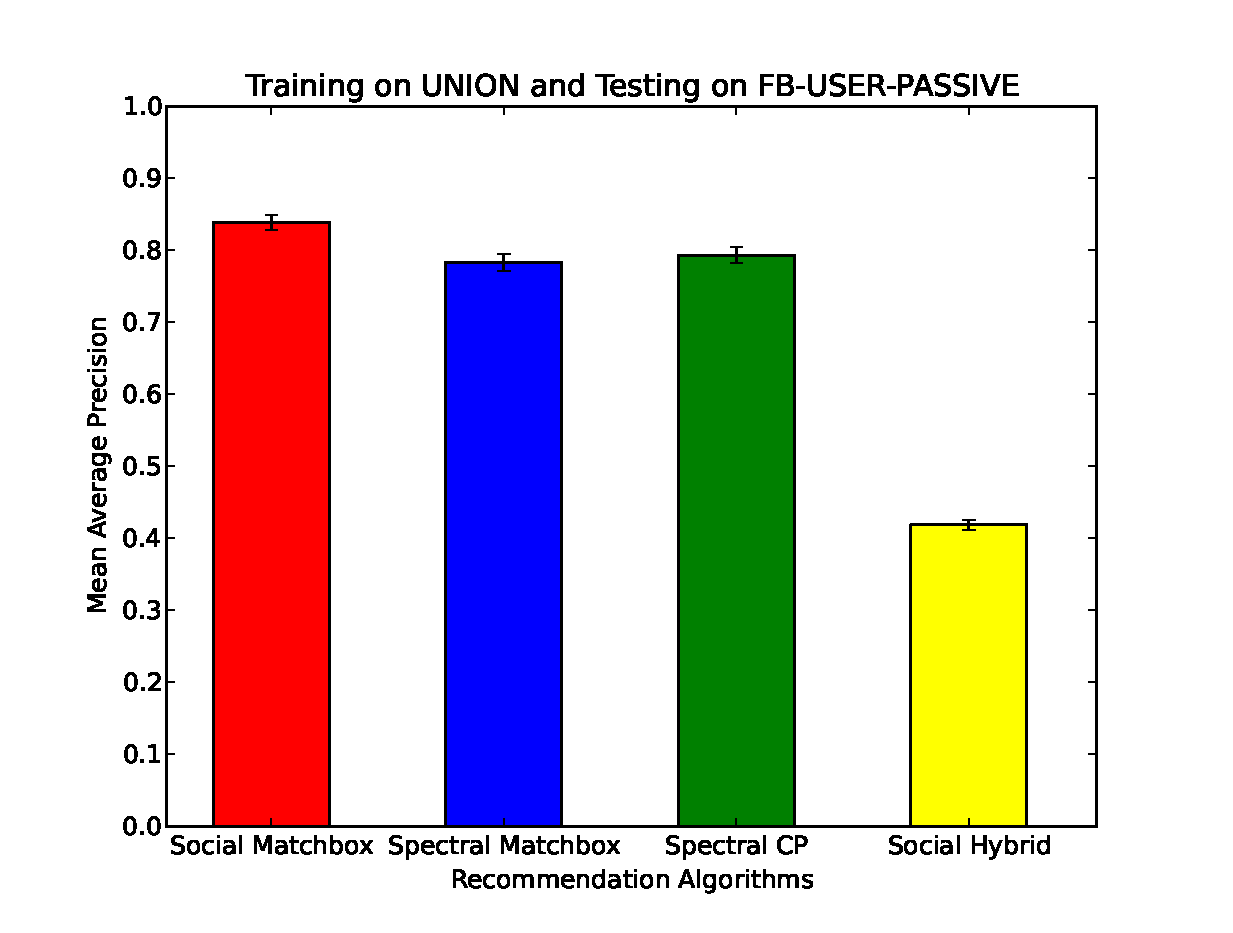
\includegraphics[scale=0.35]{img/Union_FB-User-Passive2.eps}}
\subfigure{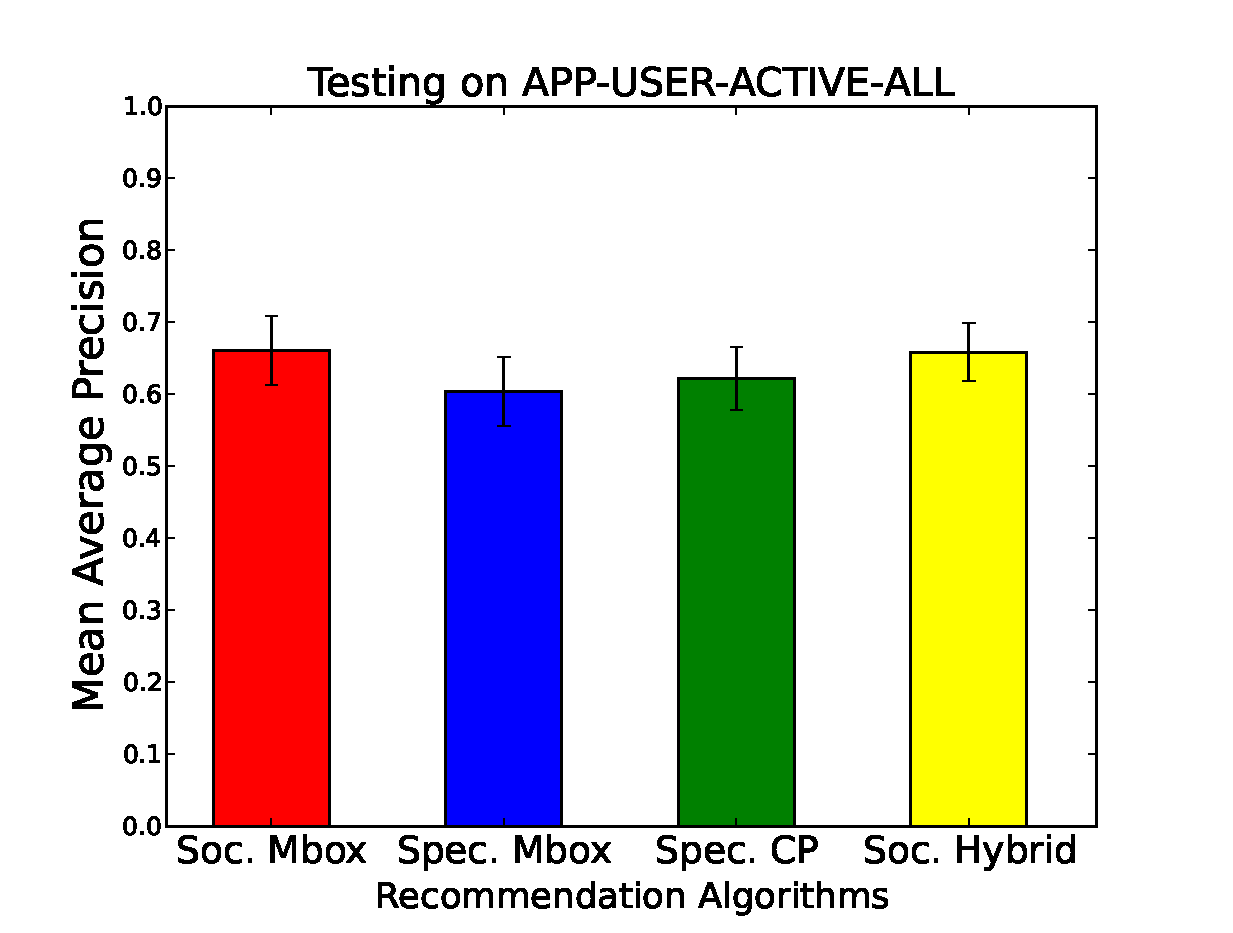
\includegraphics[scale=0.35]{img/Union_App-User-Active-All2.eps}}
\subfigure{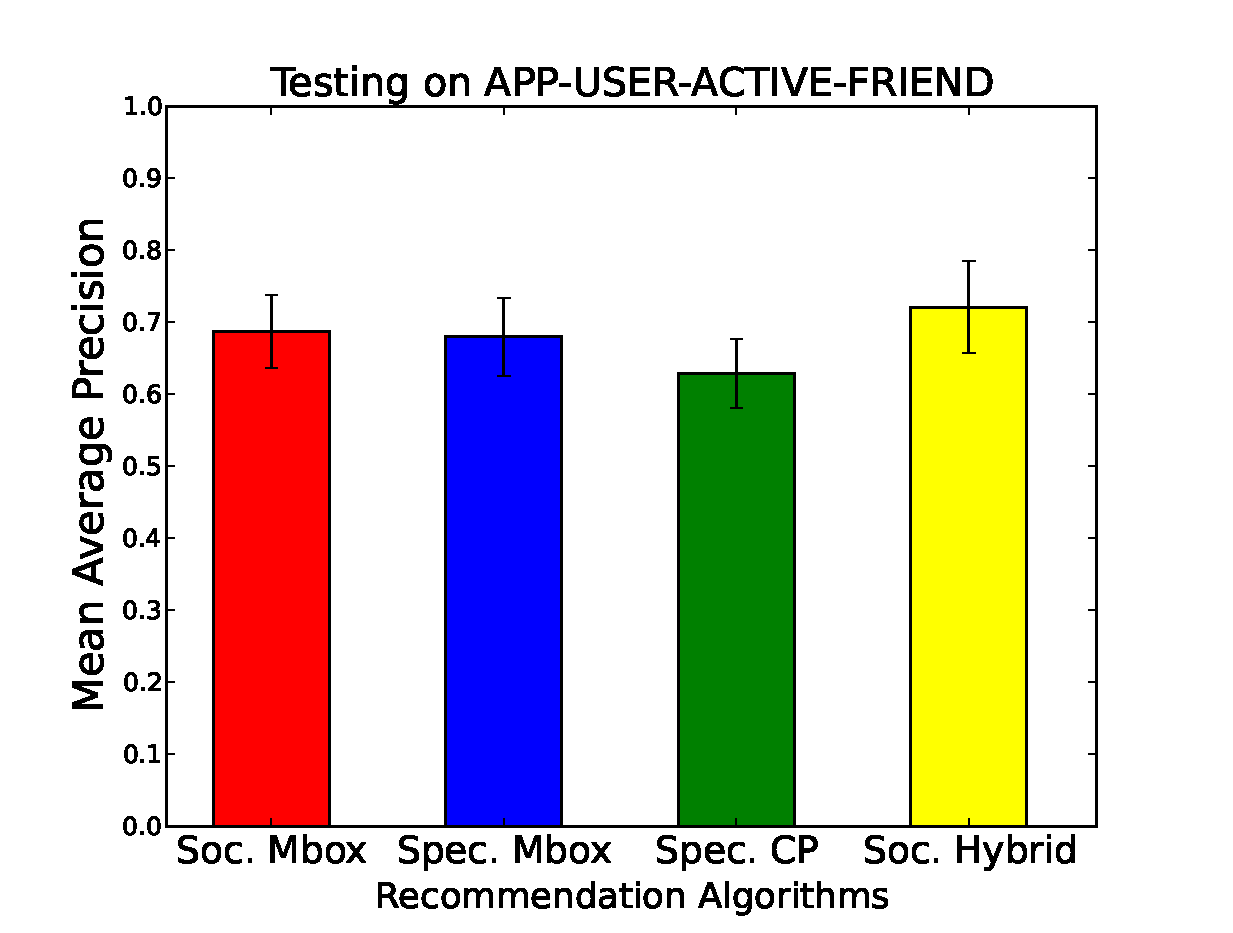
\includegraphics[scale=0.35]{img/Union_App-User-Active-Friends2.eps}}
\subfigure{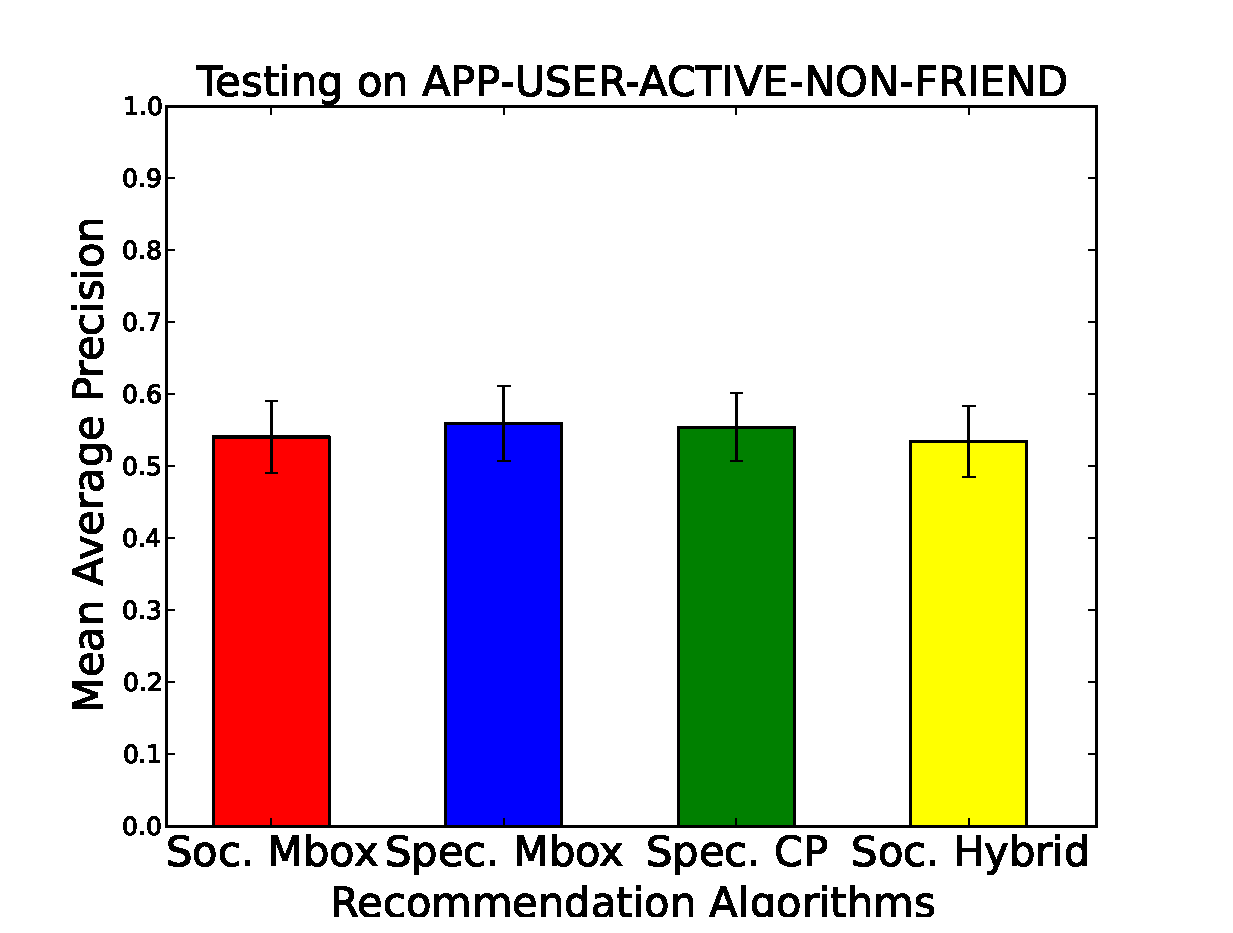
\includegraphics[scale=0.35]{img/Union_App-User-Active-NonFriends2.eps}}
\caption{Results of training on Union data}
\label{fig:union2}
\end{figure}

\section{Summary}

We summarize the observations made during the second trial:

\begin{itemize}
\item{The social spectral regularization methods generally performed better in the live user trials, even when the results were split between friend link recommendations and non-friend link recommendations.}

\item{Learning information diffusion models helps in SCF, as evidenced by the strong performance of Social Hybrid when recommending friend links.}

\item{When there is no social interaction information, learning implicit co-likes information is better than using plain CF methods.}

\item{The better performance of the social spectral regularization methods in the live trials were not reflected in the offline experiments. Perhaps there is a better metric than MAP that correlates with human preferences.}

\end{itemize}

